\mfpicnumber{1}

\opengraphsfile{Regression}

\setcounter{footnote}{0}

\label{Regression}

We have seen examples already in the text where linear and quadratic functions are used to model a wide variety of real world phenomena ranging from  production costs to the height of a projectile above the ground.  In this section, we use some basic tools from statistical analysis to quantify linear and quadratic trends that we may see in real world data in order to generate linear and quadratic models.  Our goal is to give the reader an understanding of the basic processes involved, but we are quick to refer the reader to a more advanced course\footnote{and authors with more expertise in this area,} for a complete exposition of this material.  Suppose we collected three data points: $\{(1,2), (3,1), (4,3)\}$.  By plotting these points, we can clearly see that they do not lie along the same line.  If we pick any two of the points, we can find a line containing both which completely misses the third, but our aim is to find a line which is in some sense `close' to all the points, even though it may go through none of them.  The way we measure `closeness' in this case is to find the \index{regression ! total squared error}\index{total squared error}\textbf{total squared error} between the data points and the line. Consider our three data points and the line $y=\frac{1}{2}x + \frac{1}{2}$.  For each of our data points, we find the vertical distance between the point and the line.  To accomplish this, we need to find a point on the line directly above or below each data point - in other words, a point on the line with the same $x$-coordinate as our data point.  For example, to find the point on the line directly below $(1,2)$, we plug $x=1$ into $y=\frac{1}{2}x + \frac{1}{2}$ and we get the point $(1,1)$.  Similarly, we get $(3,1)$ to correspond to $(3,2)$ and $\left(4,\frac{5}{2} \right)$ for $(4,3)$.    

\begin{center}

\begin{mfpic}[25]{-1}{5}{-1}{5}
\point[3pt]{(1,2), (1,1), (3,1), (3,2), (4,3), (4,2.5)}
\dashed \polyline{(1,1),(1,2)}
\dashed \polyline{(3,1),(3,2)}
\dashed \polyline{(4,3),(4,2.5)}
\function{0,5,0.1}{0.5*x+0.5}
\axes
\xmarks{1 step 1 until 4}
\ymarks{1 step 1 until 4}
\tlpointsep{4pt}
\tiny
\axislabels {x}{{$1$} 1, {$2$} 2, {$3$} 3, {$4$} 4}
\axislabels {y}{{$1$} 1, {$2$} 2, {$3$} 3, {$4$} 4}
\normalsize
\end{mfpic}

\end{center}

We find the total squared error $E$ by taking the sum of the squares of the differences of the $y$-coordinates of each data point and its corresponding point on the line. For the data and line above $E = (2-1)^2+(1-2)^2+\left(3-\frac{5}{2}\right)^2 = \frac{9}{4}$.  Using advanced mathematical machinery,\footnote{Like Calculus and Linear Algebra} it is possible to find the line which results in the lowest value of $E$.  This line is called the \index{regression ! least squares line}\index{least squares regression line}\index{line ! least squares regression}\textbf{least squares regression line}, or sometimes the `line of best fit'. \index{line ! of best fit} The formula for the line of best fit requires notation we won't present until Chapter \ref{Sequences}, so we will revisit it then.  The graphing calculator can come to our assistance here, since it has a built-in feature to compute the regression line.  We enter the data and perform the Linear Regression feature and we get

\begin{center}

\begin{tabular}{cc}

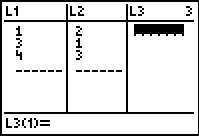
\includegraphics[width=2in]{./LinearQuadraticGraphics/RegData01.jpg} \hspace{0.75in} & 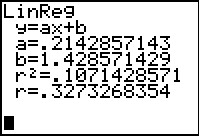
\includegraphics[width=2in]{./LinearQuadraticGraphics/RegLine01.jpg}

\end{tabular}
\end{center}

The calculator tells us that the line of best fit is $y=ax+b$ where the slope is $a \approx 0.214$ and the $y$-coordinate of the $y$-intercept is $b \approx 1.428$.  (We will stick to using three decimal places for our approximations.)  Using this line, we compute the total squared error for our data to be $E \approx 1.786$.  The value $r$ is the \index{regression ! correlation coefficient}\index{correlation coefficient}\textbf{correlation coefficient} and is a measure of how close the data is to being on the same line.  The closer $|r|$ is to $1$, the better the linear fit.  Since $r \approx 0.327$, this tells us that the line of best fit doesn't fit all that well - in other words, our data points aren't close to being linear. The value $r^2$ is called the \index{regression ! coefficient of determination}\index{coefficient of determination}\textbf{coefficient of determination} and is also a measure of the goodness of fit.\footnote{We refer the interested reader to a course in Statistics to explore the significance of $r$ and $r^2$.}  Plotting the data with its regression line results in the picture below.

\begin{center}  

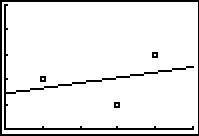
\includegraphics[width=2in]{./LinearQuadraticGraphics/RegLinePlot01.jpg}

\end{center}

Our first example looks at energy consumption in the US over the past 50 years.\footnote{See this \href{http://www.eia.doe.gov/kids/classactivities/EnergyAnalysisEIA.pdf}{\underline{Department of Energy}} activity}

\[\begin{array}{|c|c|} \hline
\mbox{Year} & \mbox{Energy Usage,} \\
& \mbox{ in Quads\footnotemark} \\ \hline
1950 & 34.6 \\ \hline
1960 & 45.1 \\ \hline
1970 & 67.8 \\ \hline
1980 & 78.3 \\ \hline
1990 & 84.6 \\ \hline
2000 & 98.9 \\ \hline

\end{array}\]
\footnotetext{The unit 1 Quad is 1 Quadrillion = $10^{15}$ BTUs, which is enough heat to raise Lake Erie roughly $1^{\circ}$F}

\begin{ex}  \label{energyconsumption}  Using the energy consumption data given above,

\begin{enumerate}

\item  Plot the data using a graphing calculator.

\item  Find the least squares regression line and comment on the goodness of fit.

\item  Interpret the slope of the line of best fit.

\item  Use the regression line to predict the annual US energy consumption in the year $2013$.

\item  Use the regression line to predict when the annual consumption will reach $120$ Quads.

\end{enumerate}

{\bf Solution.}

\begin{enumerate}


\item  Entering the data into the calculator gives

\begin{center}

\begin{tabular}{cc}

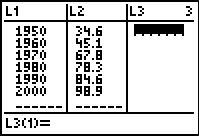
\includegraphics[width=2in]{./LinearQuadraticGraphics/RegData02.jpg} \hspace{0.75in} & 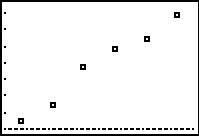
\includegraphics[width=2in]{./LinearQuadraticGraphics/RegDataPlot02.jpg}

\end{tabular}

\end{center}

The data certainly appears to be linear in nature.

\item  Performing a linear regression produces


\begin{center}

\begin{tabular}{cc}

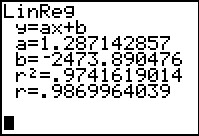
\includegraphics[width=2in]{./LinearQuadraticGraphics/RegLine02.jpg} \hspace{0.75in} & 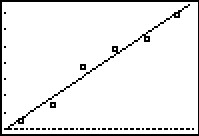
\includegraphics[width=2in]{./LinearQuadraticGraphics/RegLinePlot02.jpg}

\end{tabular}

\end{center}

We can tell both from the correlation coefficient as well as the graph that the regression line is a good fit to the data.

\item  The slope of the regression line is $a \approx 1.287$.  To interpret this, recall that the slope is the rate of change of the $y$-coordinates with respect to the $x$-coordinates.  Since the $y$-coordinates represent the energy usage in Quads, and the $x$-coordinates represent years, a slope of positive $1.287$ indicates an increase in annual energy usage at the rate of $1.287$ Quads per year.

\item  To predict the energy needs in $2013$, we substitute $x=2013$ into the equation of the line of best fit to get  $y = 1.287(2013)-2473.890 \approx 116.841$.  The predicted annual energy usage of the US in $2013$ is approximately $116.841$ Quads.

\item  To predict when the annual US energy usage will reach $120$ Quads, we substitute $y=120$ into the equation of the line of best fit to get $120 = 1.287x - 2473.908$.  Solving for $x$ yields $x \approx 2015.454$.  Since the regression line is increasing, we interpret this result as saying the annual usage in $2015$ won't yet be $120$ Quads, but that in $2016$, the demand will be more than $120$ Quads. \qed

\end{enumerate}
\end{ex}

Our next example gives us an opportunity to find a nonlinear model to fit the data.  According to the National Weather Service, the predicted hourly temperatures for Painesville on March 3, 2009 were given as summarized below.

\[\begin{array}{|c|c|} \hline
\mbox{Time} & \mbox{Temperature, $^{\circ}$F} \\ \hline
10 \mbox{AM} & 17 \\ \hline
11 \mbox{AM} & 19 \\ \hline
12 \mbox{PM} & 21 \\ \hline
1 \mbox{PM} & 23 \\ \hline
2 \mbox{PM} & 24 \\ \hline
3 \mbox{PM} & 24 \\ \hline
4 \mbox{PM} & 23 \\ \hline

\end{array}\]

To enter this data into the calculator, we need to adjust the $x$ values, since just entering the numbers could cause confusion. (Do you see why?)  We have a few options available to us.  Perhaps the easiest is to convert the times into the 24 hour clock time so that $1$ PM is $13$, $2$ PM is $14$, etc..  If we enter these data into the graphing calculator and plot the points we get

\begin{center}

\begin{tabular}{cc}

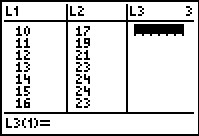
\includegraphics[width=2in]{./LinearQuadraticGraphics/RegData03.jpg} \hspace{0.75in} & 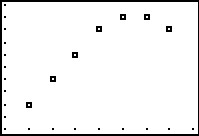
\includegraphics[width=2in]{./LinearQuadraticGraphics/RegPlot03.jpg}

\end{tabular}

\end{center}

While the beginning of the data looks linear, the temperature begins to fall in the afternoon hours.  This sort of behavior reminds us of parabolas, and, sure enough, it is possible to find a parabola of best fit in the same way we found a line of best fit.  The process is called \index{regression ! quadratic}\index{quadratic regression}\textbf{quadratic regression} and its goal is to minimize the least square error of the data with their corresponding points on the parabola.  The calculator has a built in feature for this as well which yields

\begin{center}

\begin{tabular}{cc}

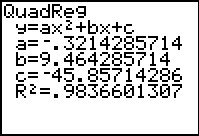
\includegraphics[width=2in]{./LinearQuadraticGraphics/RegPara03.jpg} \hspace{0.75in} & 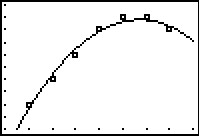
\includegraphics[width=2in]{./LinearQuadraticGraphics/RegParaPlot03.jpg}

\end{tabular}

\end{center}

The coefficient of determination $R^2$ seems reasonably close to $1$, and the graph visually seems to be a decent fit.  We use this model in our next example.

\begin{ex}  Using the quadratic model for the temperature data above, predict the warmest temperature of the day.  When will this occur?

\smallskip

{\bf Solution.}  The maximum temperature will occur at the vertex of the parabola.  Recalling the Vertex Formula, Equation \ref{vertexofquadraticfunctions}, $x = -\frac{b}{2a} \approx - \frac{9.464}{2(-0.321)} \approx 14.741$.  This corresponds to roughly $2\!:\!45$ PM.  To find the temperature, we substitute $x = 14.741$ into $y = -0.321 x^2+9.464x - 45.857$ to get $y \approx 23.899$, or $23.899^{\circ}$F.  \qed

\end{ex}

The results of the last example should remind you that regression models are just that, models.  Our predicted warmest temperature was found to be $23.899^{\circ}$F, but our data says it will warm to $24^{\circ}$F.  It's all well and good to observe trends and guess at a model, but a more thorough investigation into \emph{why} certain data should be linear or quadratic in nature is usually in order - and that, most often, is the business of scientists.

\newpage

\subsection{Exercises}

\begin{enumerate}

\item According to this \href{http://www.ohiobiz.com/census/Lake.pdf}{\underline{website}}\footnote{\href{http://www.ohiobiz.com/census/Lake.pdf}{\underline{http://www.ohiobiz.com/census/Lake.pdf}}}, the census data for Lake County, Ohio is:

\noindent \begin{tabular}{|l|r|r|r|r|} \hline
Year & 1970 & 1980 & 1990 & 2000 \\ 
\hline 
Population & 197200 & 212801 & 215499 & 227511 \\ \hline
\end{tabular}

\begin{enumerate}
 

\item  Find the least squares regression line for these data and comment on the goodness of fit.\footnote{We'll develop more sophisticated models for the growth of populations in Chapter \ref{ExpLogs}.  For the moment, we use a theorem from Calculus to approximate those functions with lines.} Interpret the slope of the line of best fit.

\item  Use the regression line to predict the population of Lake County in 2010.  (The recorded figure from the 2010 census is $230,\!041$)

\item  Use the regression line to predict when the population of Lake County will reach $250,\!000$.

\end{enumerate}


\item According to this \href{http://www.ohiobiz.com/census/Lorain.pdf}{\underline{website}}\footnote{\href{http://www.ohiobiz.com/census/Lorain.pdf}{\underline{http://www.ohiobiz.com/census/Lorain.pdf}}}, the census data for Lorain County, Ohio is:

\noindent \begin{tabular}{|l|r|r|r|r|} \hline
Year & 1970 & 1980 & 1990 & 2000 \\ 
\hline 
Population & 256843 & 274909 & 271126 & 284664 \\ \hline
\end{tabular}

\begin{enumerate}
 

\item  Find the least squares regression line for these data and comment on the goodness of fit. Interpret the slope of the line of best fit.

\item  Use the regression line to predict the population of Lorain County in 2010.  (The recorded figure from the 2010 census is $301,\!356$)

\item  Use the regression line to predict when the population of Lake County will reach $325,\!000$.

\end{enumerate}
\item Using the energy production data given below

\noindent \begin{tabular}{|l|r|r|r|r|r|r|} \hline
Year & 1950 & 1960 & 1970 & 1980 & 1990 & 2000 \\ 
\hline 
Production & & & & & & \\
(in Quads) & 35.6 & 42.8 & 63.5 & 67.2 & 70.7 & 71.2 \\ \hline
\end{tabular}

\begin{enumerate}

\item  Plot the data using a graphing calculator and explain why it does not appear to be linear.

\item  Discuss with your classmates why ignoring the first two data points may be justified from a historical perspective.  

\item Find the least squares regression line for the last four data points and comment on the goodness of fit. Interpret the slope of the line of best fit.

\item  Use the regression line to predict the annual US energy production in the year $2010$.

\item  Use the regression line to predict when the annual US energy production will reach $100$ Quads.

\end{enumerate}


\item The chart below contains a portion of the fuel consumption information for a 2002 Toyota Echo that I (Jeff) used to own.  The first row is the cumulative number of gallons of gasoline that I had used and the second row is the odometer reading when I refilled the gas tank.  So, for example, the fourth entry is the point (28.25, 1051) which says that I had used a total of 28.25 gallons of gasoline when the odometer read 1051 miles.

\medskip

\small

\noindent \begin{tabular}{|l|r|r|r|r|r|r|r|r|r|r|r|} \hline
Gasoline Used & & & & & & & & & & & \\
(Gallons)  & 0 & 9.26 & 19.03 & 28.25 & 36.45 & 44.64 & 53.57 & 62.62 & 71.93 & 81.69 & 90.43\\ 
\hline 
Odometer & & & & & & & & & & & \\
(Miles) & 41 & 356 & 731 & 1051 & 1347 & 1631 & 1966 & 2310 & 2670 & 3030 & 3371\\ \hline
\end{tabular}

\normalsize

\medskip

\noindent Find the least squares line for this data.  Is it a good fit?  What does the slope of the line represent?  Do you and your classmates believe this model would have held for ten years had I not crashed the car on the Turnpike a few years ago?  (I'm keeping a fuel log for my 2006 Scion xA for future College Algebra books so I hope not to crash it, too.)

\item On New Year's Day, I (Jeff, again) started weighing myself every morning in order to have an interesting data set for this section of the book.  (Discuss with your classmates if that makes me a nerd or a geek.  Also, the professionals in the field of weight management strongly discourage weighing yourself every day.  When you focus on the number and not your overall health, you tend to lose sight of your objectives.  I was making a noble sacrifice for science, but you should \underline{not} try this at home.)  The whole chart would be too big to put into the book neatly, so I've decided to give only a small portion of the data to you.  This then becomes a Civics lesson in honesty, as you shall soon see.  There are two charts given below.  One has my weight for the first eight Thursdays of the year (January 1, 2009 was a Thursday and we'll count it as Day 1.) and the other has my weight for the first 10 Saturdays of the year.  

\medskip

\small

\noindent \begin{tabular}{|l|r|r|r|r|r|r|r|r|} \hline
Day \# & & & & & & & &  \\
(Thursday) & 1 & 8 & 15 & 22 & 29 & 36 & 43 & 50 \\ 
\hline 
My weight & & & & & & & & \\
in pounds & 238.2 & 237.0 & 235.6 & 234.4 & 233.0 & 233.8 & 232.8 & 232.0\\ \hline
\end{tabular}

\medskip

\noindent \begin{tabular}{|l|r|r|r|r|r|r|r|r|r|r|} \hline
Day \# & & & & & & & & & & \\
(Saturday) & 3 & 10 & 17 & 24 & 31 & 38 & 45 & 52 & 59 & 66 \\ 
\hline 
My weight & & & & & & & & & & \\
in pounds & 238.4 & 235.8 & 235.0 & 234.2 & 236.2 & 236.2 & 235.2 & 233.2 & 236.8 & 238.2\\ \hline
\end{tabular}

\normalsize

\medskip

\begin{enumerate}

\item Find the least squares line for the Thursday data and comment on its goodness of fit.
\item Find the least squares line for the Saturday data and comment on its goodness of fit.
\item Use Quadratic Regression to find a parabola which models the Saturday data and comment on its goodness of fit.
\item Compare and contrast the predictions the three models make for my weight on January 1, 2010 (Day \#366).  Can any of these models be used to make a prediction of my weight 20 years from now?  Explain your answer.
\item Why is this a Civics lesson in honesty?  Well, compare the two linear models you obtained above.  One was a good fit and the other was not, yet both came from careful selections of real data.  In presenting the tables to you, I have not lied about my weight, nor have you used any bad math to falsify the predictions.  The word we're looking for here is `disingenuous'.  Look it up and then discuss the implications this type of data manipulation could have in a larger, more complex, politically motivated setting.  (Even Obi-Wan presented the truth to Luke only ``from a certain point of view.'')

\end{enumerate}

\item (Data that is neither linear nor quadratic.)  We'll close this exercise set with two data sets that, for reasons presented later in the book, cannot be modeled correctly by lines or parabolas.  It is a good exercise, though, to see what happens when you attempt to use a linear or quadratic model when it's not appropriate.

\begin{enumerate}

\item \label{APLcats} This first data set came from a Summer 2003 publication of the Portage County Animal Protective League called ``Tattle Tails''.  They make the following statement and then have a chart of data that supports it. ``It doesn't take long for two cats to turn into 80 million.  If two cats and their surviving offspring reproduced for ten years, you'd end up with 80,399,780 cats.''  We assume $N(0) = 2$.

\medskip

\scriptsize

\noindent \begin{tabular}{|l|r|r|r|r|r|r|r|r|r|r|} \hline
Year $x$ & 1 & 2 & 3 & 4 & 5 & 6 & 7 & 8 & 9 & 10 \\ 
\hline 
Number of  & & & & & & & & & & \\
Cats $N(x)$ & 12 & 66 & 382 & 2201 & 12680 & 73041 & 420715 & 2423316 & 13968290 & 80399780 \\ \hline
\end{tabular}

\normalsize

\medskip

\noindent Use Quadratic Regression to find a parabola which models this data and comment on its goodness of fit. (Spoiler Alert: Does anyone know what type of function we need here?)

\medskip

\item \label{regsunlight} This next data set comes from the \href{http://aa.usno.navy.mil/data/docs/RS_OneYear.php}{\underline{U.S. Naval Observatory}}.  That site has loads of awesome stuff on it, but for this exercise I used the sunrise/sunset times in Fairbanks, Alaska for 2009 to give you a chart of the number of hours of daylight they get on the $21^{\mbox{st}}$ of each month.  We'll let $x = 1$ represent January 21, 2009, $x = 2$ represent February 21, 2009, and so on.

\medskip

\small

\noindent \begin{tabular}{|l|r|r|r|r|r|r|r|r|r|r|r|r|} \hline
Month  & & & & & & & & & & & & \\
Number & 1 & 2 & 3 & 4 & 5 & 6 & 7 & 8 & 9 & 10 & 11 & 12\\ 
\hline 
Hours of  & & & & & & & & & & & & \\
Daylight & 5.8 & 9.3 & 12.4 & 15.9 & 19.4 & 21.8 & 19.4 & 15.6 & 12.4 & 9.1 & 5.6 & 3.3 \\ \hline
\end{tabular}

\normalsize

\medskip

\noindent Use Quadratic Regression to find a parabola which models this data and comment on its goodness of fit. (Spoiler Alert: Does anyone know what type of function we need here?)

\end{enumerate}

\end{enumerate}

\newpage

\subsection{Answers}

\begin{enumerate}

\item  \begin{enumerate}
 

\item  $y = 936.31x - 1645322.6$ with $r=0.9696$ which indicates a good fit.  The slope $936.31$ indicates Lake County's population is increasing at a rate of (approximately) 936 people per year. 

\item  According to the model, the population in 2010 will be $236, \!660$.

\item  According to the model, the population of Lake County will reach $250,\!000$ sometime between 2024 and 2025.

\end{enumerate}

\item  \begin{enumerate}
 

\item  $y = 796.8x - 1309762.5$ with $r=0.8916$ which indicates a reasonable fit.  The slope $796.8$ indicates Lorain County's population is increasing at a rate of (approximately) 797 people per year. 

\item  According to the model, the population in 2010 will be $291, \! 805$.

\item  According to the model, the population of Lake County will reach $325,\!000$ sometime between 2051 and 2052.

\end{enumerate}

\item \begin{enumerate}

\setcounter{enumii}{2}

\item $y = 0.266x - 459.86$ with $r = 0.9607$ which indicates a good fit.  The slope $0.266$ indicates the country's energy production is increasing at a rate of $0.266$ Quad per year.

\item According to the model, the production in 2010 will be $74.8$ Quad.

\item According to the model, the production will reach $100$ Quad in the year 2105.

\end{enumerate}

\item The line is $y = 36.8x + 16.39$.  We have $r = .99987$ and $r^{2} = .9997$ so this is an excellent fit to the data.  The slope $36.8$ represents miles per gallon.

\item \begin{enumerate}

\item The line for the Thursday data is $y = -.12x + 237.69$.  We have $r = -.9568$ and $r^{2} = .9155$ so this is a really good fit.

\item The line for the Saturday data is $y = -0.000693x + 235.94$.  We have $r = -0.008986$ and $r^{2} = 0.0000807$ which is horrible.  This data is not even close to linear.  

\item The parabola for the Saturday data is $y = 0.003x^{2} - 0.21x + 238.30$.  We have $R^{2} = .47497$ which isn't good.  Thus the data isn't modeled well by a quadratic function, either.

\item The Thursday linear model had my weight on January 1, 2010 at 193.77 pounds.  The Saturday models give 235.69 and 563.31 pounds, respectively.  The Thursday line has my weight going below 0 pounds in about five and a half years, so that's no good.  The quadratic has a positive leading coefficient which would mean unbounded weight gain for the rest of my life.  The Saturday line, which mathematically does not fit the data at all, yields a plausible weight prediction in the end.  I think this is why grown-ups talk about ``Lies, Damned Lies and Statistics.''

\end{enumerate}

\item \begin{enumerate}

\item The quadratic model for the cats in Portage county is $y = 1917803.54x^{2} - 16036408.29x + 24094857.7$.  Although $R^{2} = .70888$ this is not a good model because it's so far off for small values of $x$.  Case in point, the model gives us 24,094,858 cats when $x = 0$ but we know $N(0) = 2$.

\item The quadratic model for the hours of daylight in Fairbanks, Alaska is $y = .51x^{2} + 6.23x - .36$.  Even with $R^{2} = .92295$ we should be wary of making predictions beyond the data.  Case in point, the model gives $-4.84$ hours of daylight when $x = 13$.  So January 21, 2010 will be ``extra dark''?  Obviously a parabola pointing down isn't telling us the whole story.

\end{enumerate}

\end{enumerate}


\closegraphsfile